\section{Filastruder-sensor diámetro-Tractora}
\label{sec:FSB}

En una de las pruebas de extrusión de filamento, se va estirando a mano según va saliendo de la filastruder y se comprueba que, traccionando del hilo a una distancia cercana de la boquilla y una vez enfriado, se puede llegar a regular el diámetro final. Por ello, se trata de investigar en esta linea, diseñar un sistema capaz de traccionar el filamento a medida que va saliendo de la boquilla.

\begin{figure}[H]
    \centering
    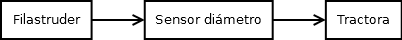
\includegraphics[width=0.6\textwidth]{images/producciones/Diagram2.png}
    \caption{Esquema de producción}
    \label{fig:esquemap_FST}
\end{figure}

Con el conocimiento adquirido al diseñar la peletizadora (ver capítulo \fullref{sec:peletizadora}) se diseña una unidad tractora que irá colocada después de la filastruder, la cual, deberá ir traccionando del filamento independientemente del diámetro del mismo. Así mismo, deberemos ser capaces de regular la velocidad de una forma más precisa que como lo hicimos con la peletizadora. El material del que dispondremos será el siguiente.

\begin{itemize}
	\item{\textbf{Arduino Mega:} Microcontrolador encargado de mover un motor y regular su velocidad.}
	\item{\textbf{RAMPS:} Placa auxiliar colocada encima del arduino Mega, la cual dispone de un driver A4988 para controlar varios motores paso a paso.}
	\item{\textbf{Motor paso a paso:} Dispositivo electromagnético, que transforma una serie de impuslos eléctricos en desplazamientos angulares.}
\end{itemize}

Se vuelve a elegir un motor paso a paso como unidad de tracción, debido a las mismas razones por las que se eligió en la peletizadora.\\

El principio de funcionamiento de un motor paso a paso es sencillo. En el interior del mismo se dispone de dos bobinas giradas 90º entre sí \cite{pasoapaso} las cuales, en función de una secuencia de excitación, generarán campos magnéticos que hará que el rotor del mismo giré un determinado ángulo. Para la realización de la tractora, se usará una ténica denominada de micropasos con la que conseguimos que nuestro motor de 1.8º de giro pueda alcanzazr grados de 0.225º. Para poder controlar el motor con está técnica y conseguir una velocidad de rotación constante, será necesario que el microcontrolador genera una señal cuadrada, en la que dependiendo de la frecuencia de esta señal, el motor girará a una velocidad distinta. El nivel alto de esta señal cuadrada, se la denominará paso. Por cada paso que reciba el motor, girará $1.8º$ dividido el número de micropasos configurados en el driver:

\begin{table}[H]
    \centering
    \begin{tabular}{cccc}
        {\bf MS1} & {\bf MS2} & {\bf MS3} & {\bf Resolución de micropaso}  \\
        \hline
        L         & L         & L         & Paso completo (1)              \\
        H         & L         & L         & Medio paso (1/2)               \\
        L         & H         & L         & Un cuarto de paso (1/4)        \\
        H         & H         & L         & Un octavo de paso (1/8)        \\
        H         & H         & H         & Un dieciseisavo de paso (1/16)
    \end{tabular}
    \caption{Resolución del driver en función del micropaso elegido}
    \label{tab:res_drive}
\end{table}

Para el caso que nos ocupa, elegiremos la configuración de un dieciseisavo de resolución,es decir:

$$ \text{Pasos por vuelta} = \frac{360º}{1.8º \cdot \frac{1}{16} } = 3200 \text{pasos}  $$

Por tanto, si quisieramos girar el motor a una velocidad de $1RPM$ tendríamos que da un total de:

$$\frac{1 RPM \cdot 3200 pasos}{60 s} = 53 pasos/s$$

O lo que es lo mismo, un paso cada $18.86 ms$. Esta separación temporal, va inversamente relacionada con la velocidad de giro deseada, cuanta más velocidad de giro queramos, menor será el tiempo entre pasos. Para poder generar el tren de pulsos, se usará una interrupción del mirocontrolador, que se ejecutará cada $10\mu s$ e irá incrementando un contador, el cual, al llegar a un valor máximo determinado por la velocidad de giro, efectuará un escalón. El valor máximo del contador viene dado por la fórmula:

$$ Valor_{Max} = \frac{\text{Separación temporal de ticks}}{\text{Tiempo de interrupción}}$$

En nuestro caso, para girar el motor a una velocidad de 1RPM con una interrupción de $10\mu s$ deberíamos contar el siguiente número:

$$Valor_{Max} = \frac{18.75 ms}{10\mu s} = 1875$$

Por especificación del filastruder, determinamos que la velocidad de tracción deberá ir entre el rango de 1RPM y 3RPM, por tanto, con ayuda de una hoja de cálculo de excel, determinamos los valores máximosa a contar en función de la velocidad de giro.

\begin{table}[H]
    \centering
    \begin{tabular}{cccc}
        \multicolumn{1}{l}{{\bf RPM}} & \multicolumn{1}{l}{{\bf TICKS/S}} & \multicolumn{1}{l}{{\bf Separacion ticks (s)}} & \multicolumn{1}{l}{{\bf Ticks a contar por ISR}} \\
        \hline
        0 & -1 & -1 & -1 \\
        1 & 53 & 0,01875 & 1875 \\
        2 & 107 & 0,009375 & 938 \\
        3 & 160 & 0,00625 & 625
    \end{tabular}
    \caption{Valores para controla la velocidad de giro del motor paso a paso}
    \label{tab:valores_paso_paso}
\end{table}

Por tanto, cuando el contador llegue a los valores máximos establecidos, se generará un pulso, haciendo que el motor avance los grados determinados. A su vez, la velocidad de giro, vendrá dada por el PLC el cual, en función de un tensión de 0 a 5 V hará que el motor giré a una velocidad distinta.\\

Una vez establecida la arquitectura del software, se pasa a diseñar las piezas necesarias para crear la unidad tractora. Como la vez anterior, usaremos la herramienta Autodesk Inventor. Como unidad tractora, se diseñará una pieza que irá acoplado al eje de giro del motor, la cual irá recubierta por una goma para aumentar la fricción con el filamento. Con ayuda de un rodamiento haciendo presión por la otra parte del filamento, conseguiremos que se desplace de forma lineal

\begin{figure}[H]
    \centering
    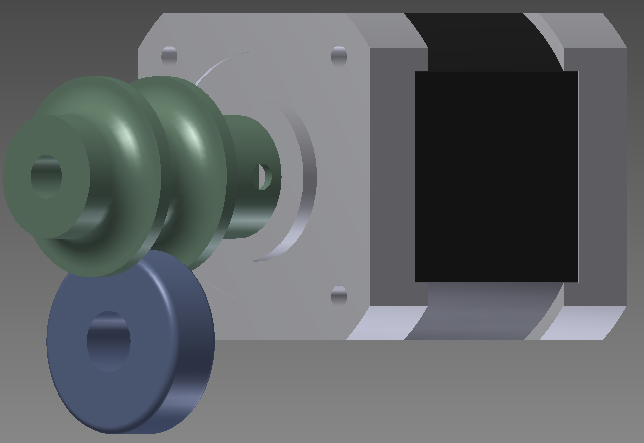
\includegraphics[width=0.6\textwidth]{images/producciones/tractora/motor.png}
    \caption{Diseño del eje de giro de la tractora}
    \label{fig:tractora}
\end{figure}


La pieza que soporte el rodamiento, deberá ir apretada por un muelle, para conseguir que asuma los cambios de diámetro y pueda hacer desplazar cualquier filamento sin importar el diámetro.

\begin{figure}[H]
    \centering
    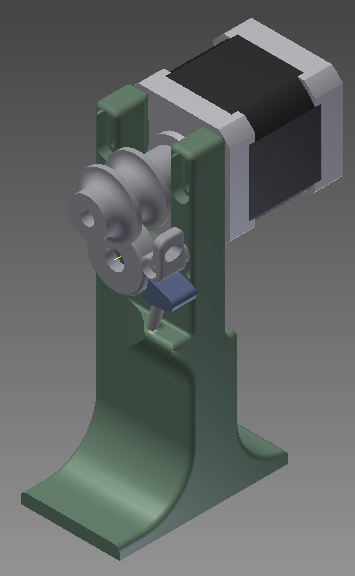
\includegraphics[width=0.5\textwidth]{images/producciones/tractora/asembli.png}
    \caption{Diseño de la tractora}
    \label{fig:tractora2}
\end{figure}

Una vez diseñadas las piezas, se pasan a imprimir en una impresora 3D

\begin{figure}[H]
    \centering
    \begin{subfigure}[b]{0.3\textwidth}
        \centering
        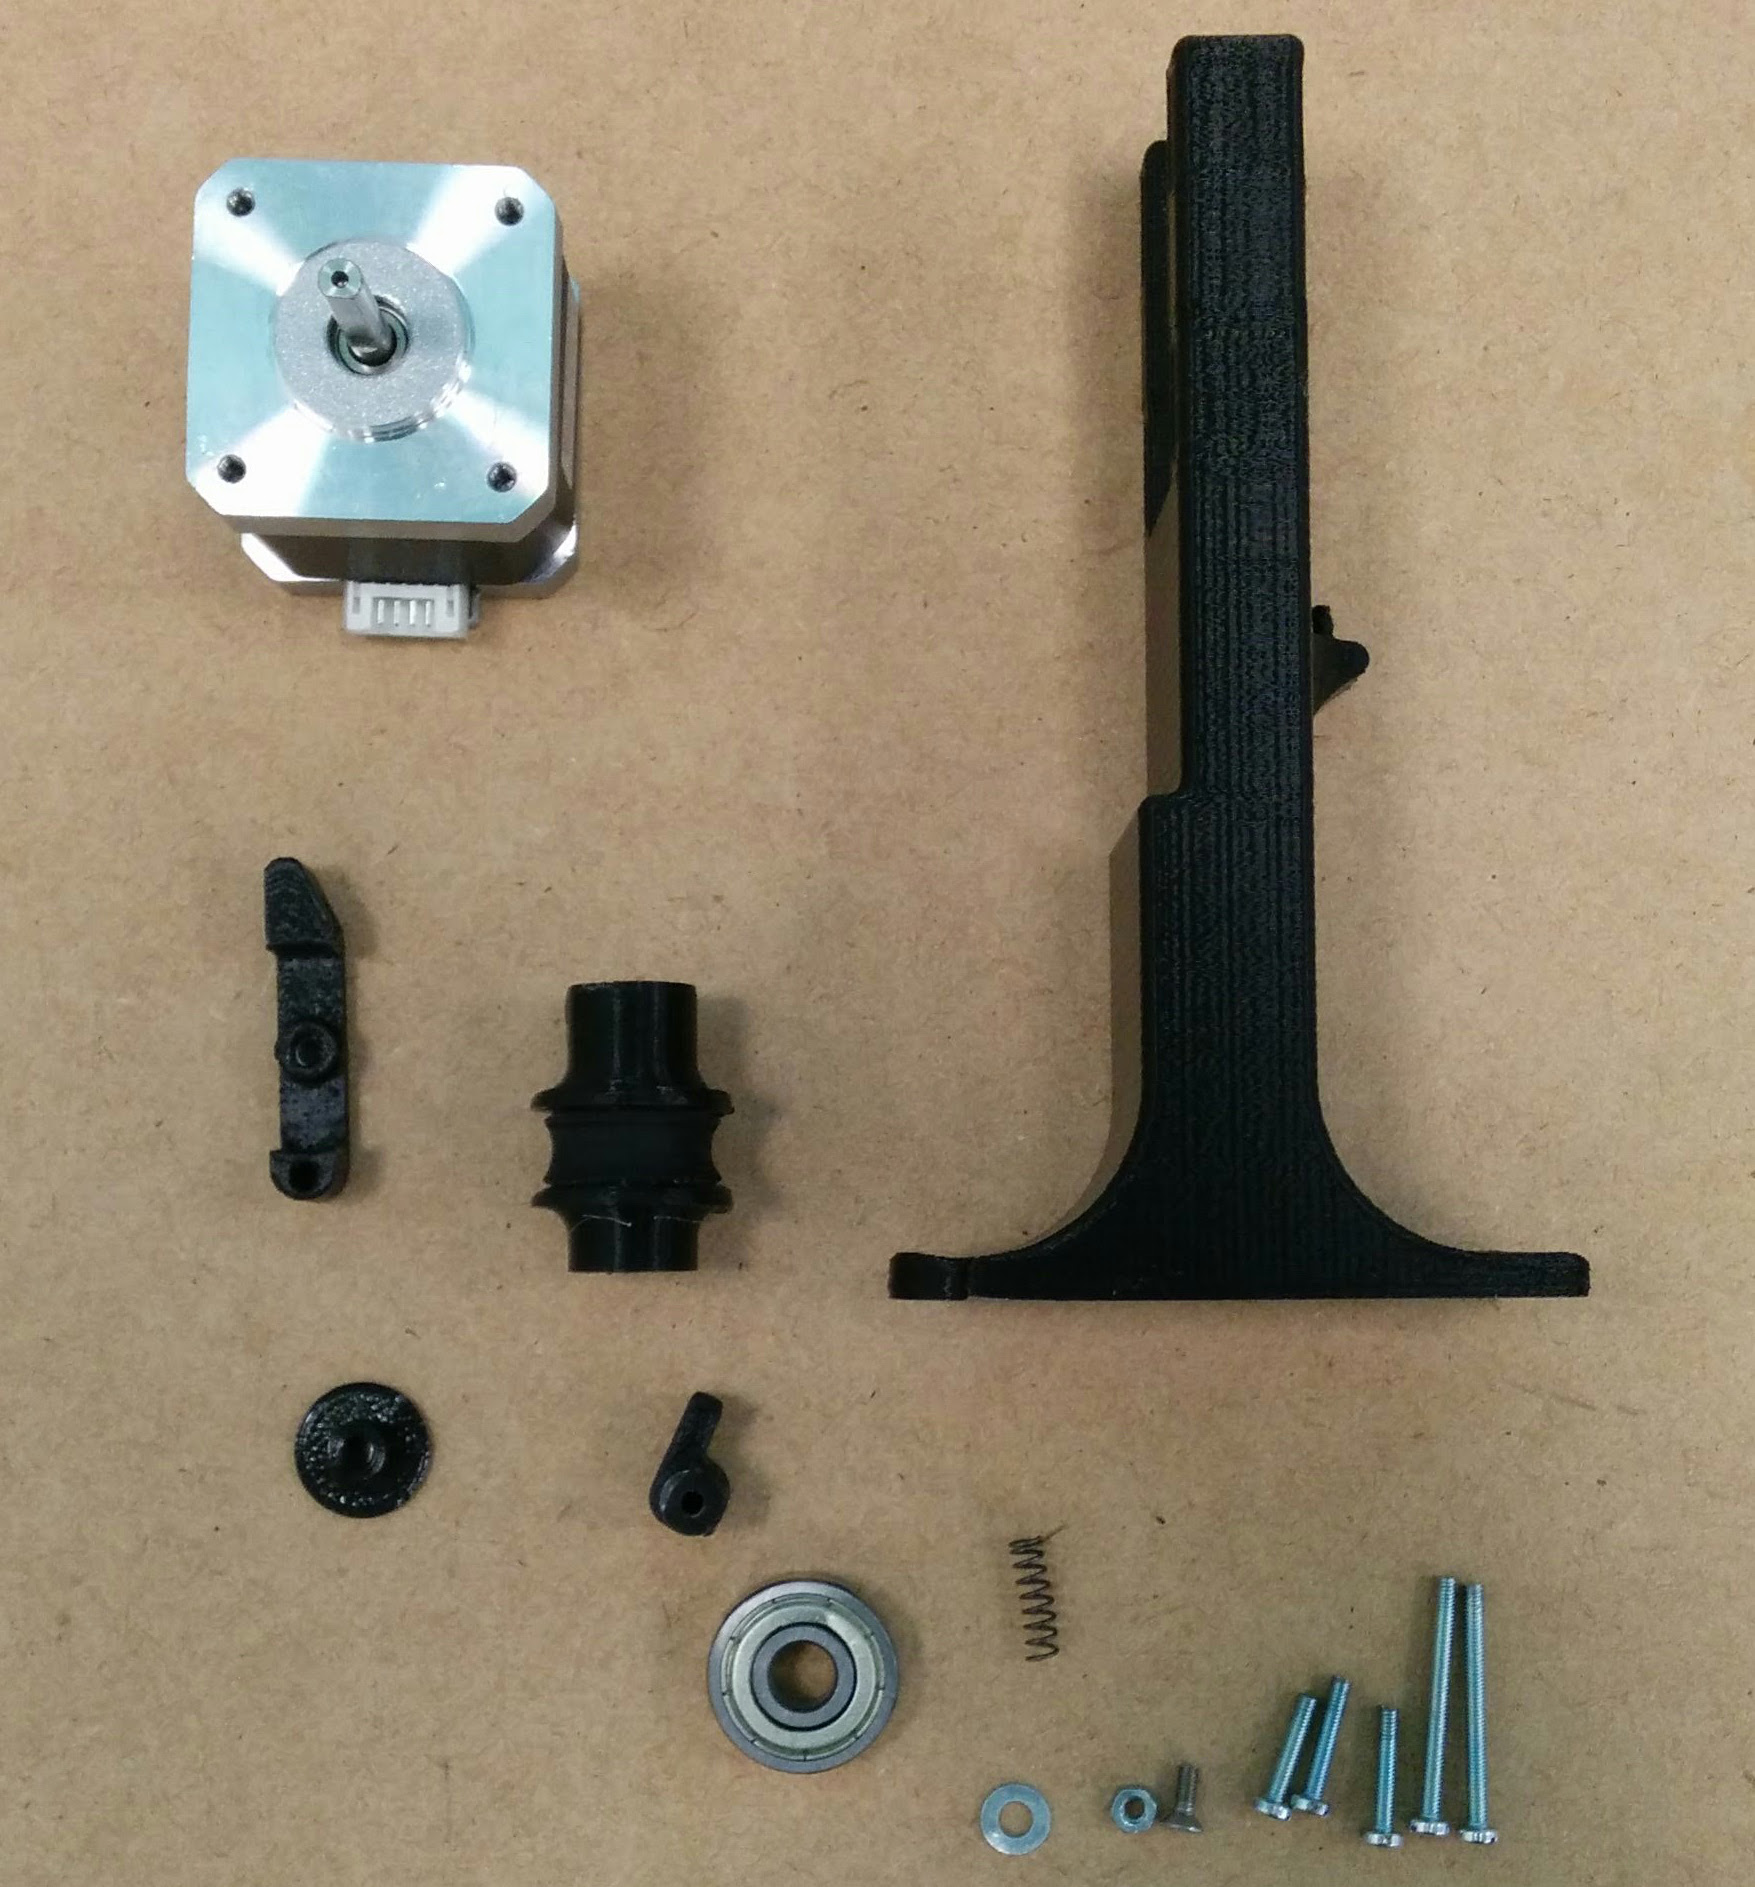
\includegraphics[width=\linewidth]{images/producciones/tractora/IMG_20150804_085937.jpg}
        \caption{Piezas impresoras de la tractora}
        \label{fig:tractora_piezas}
    \end{subfigure}
    ~
    \begin{subfigure}[b]{0.3\textwidth}
            \centering
        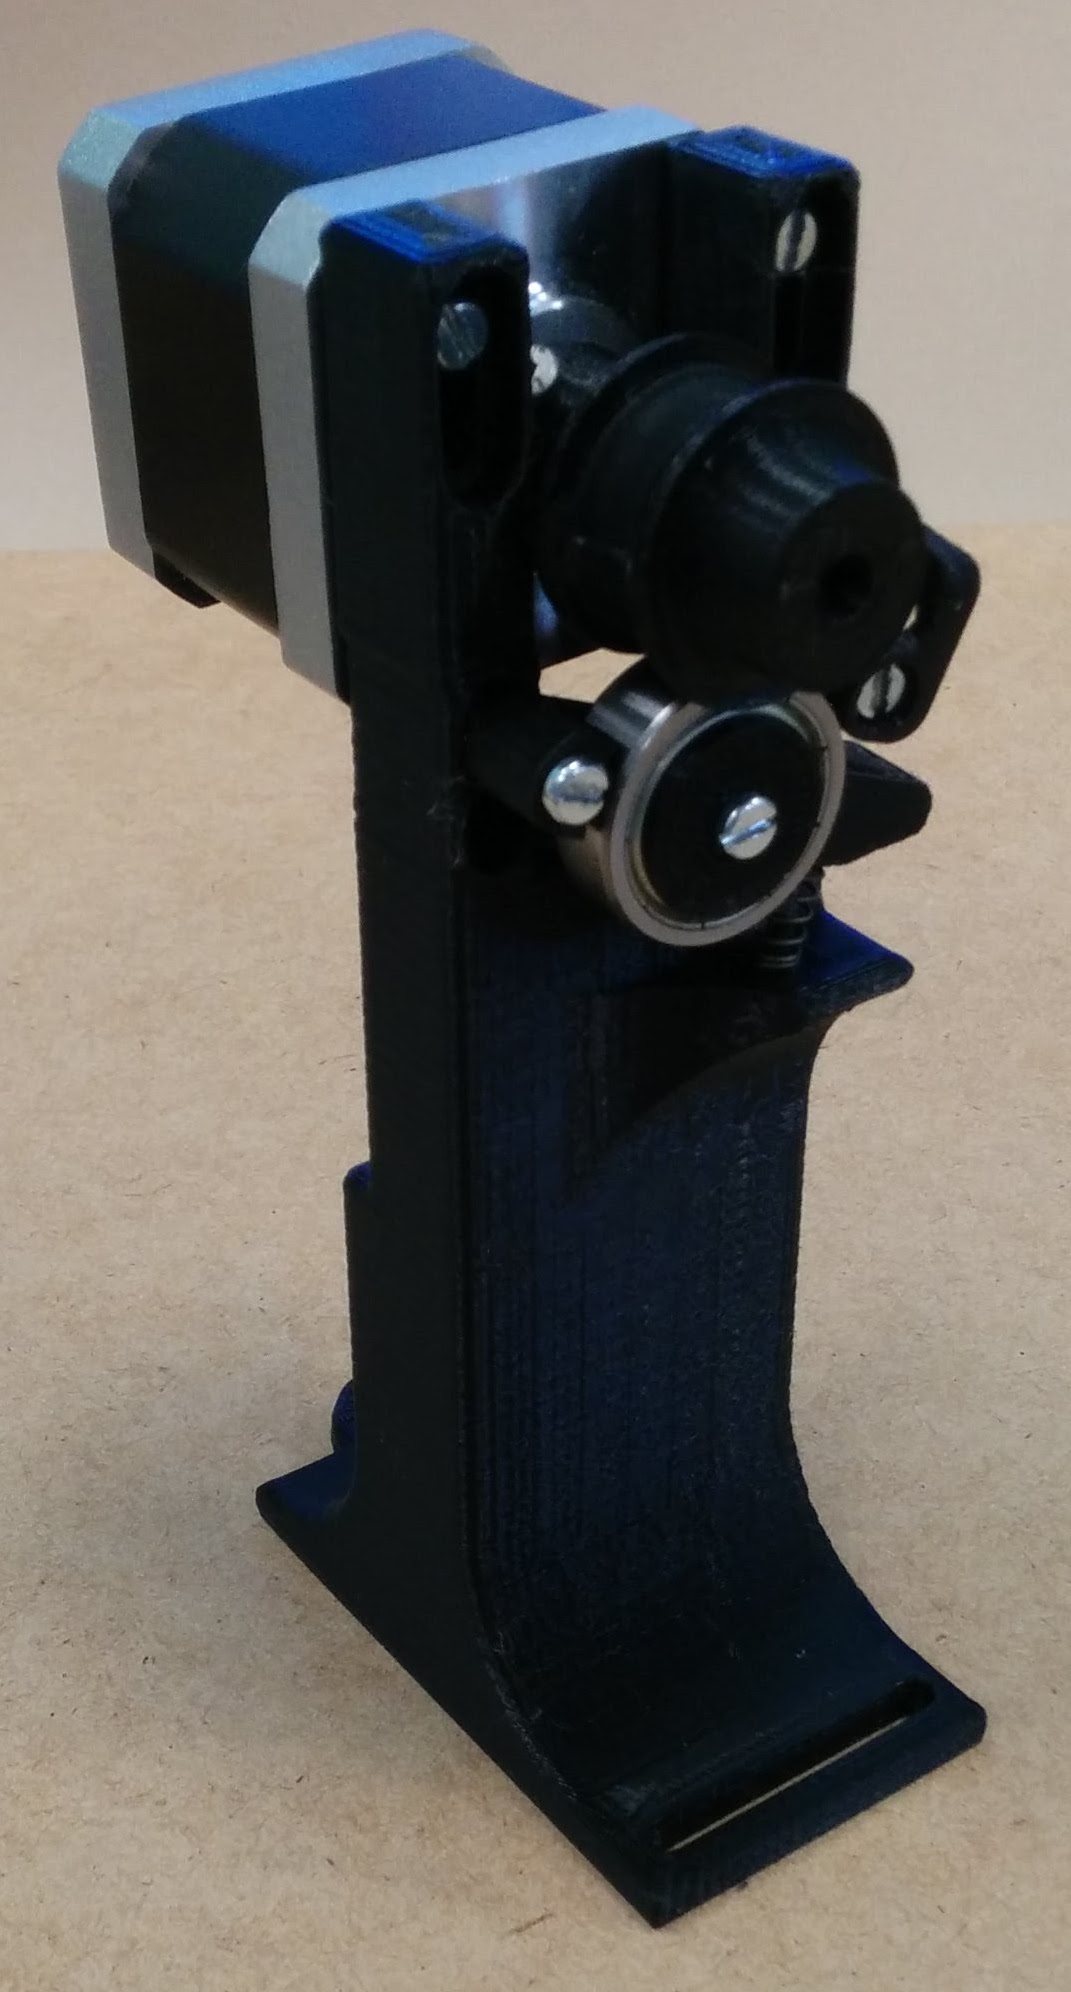
\includegraphics[width=\linewidth]{images/producciones/tractora/IMG_20150804_090625.jpg}
        \caption{Tractora montada}
        \label{fig:tractora_montada}
    \end{subfigure}
    \caption{Pieza de la tractora.}
    \label{fig:tractora_montaj}
\end{figure}

Por último, para comprobar que el funcionamiento de la tractora es el esperado, se hace pasar una bobina de filamento através de la tractora, y comprobamos que podemos variar la velocidad de tracción y el agarre del filamento es el adecuado.

	\begin{figure}[H]
            \centering
            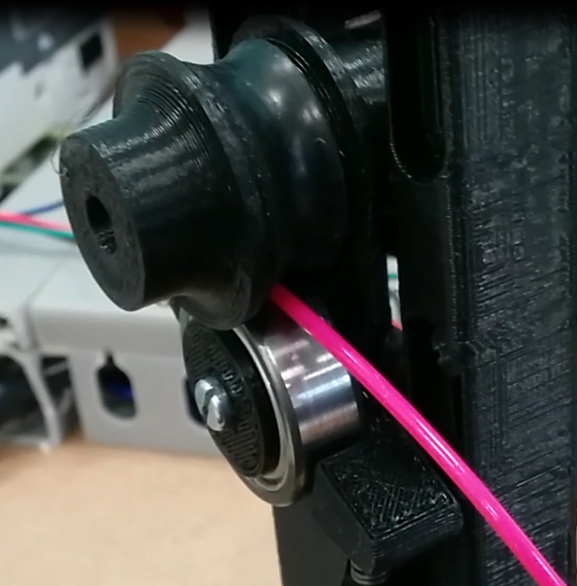
\includegraphics[width=0.5\textwidth]{images/producciones/tractora/final.png}
            \caption{Tractora con filamento}
            \label{fig:tractora_fila}
    \end{figure}


Por tanto, podemos pasar a instalar la tractora en la maqueta.

\begin{figure}[H]
    \centering
    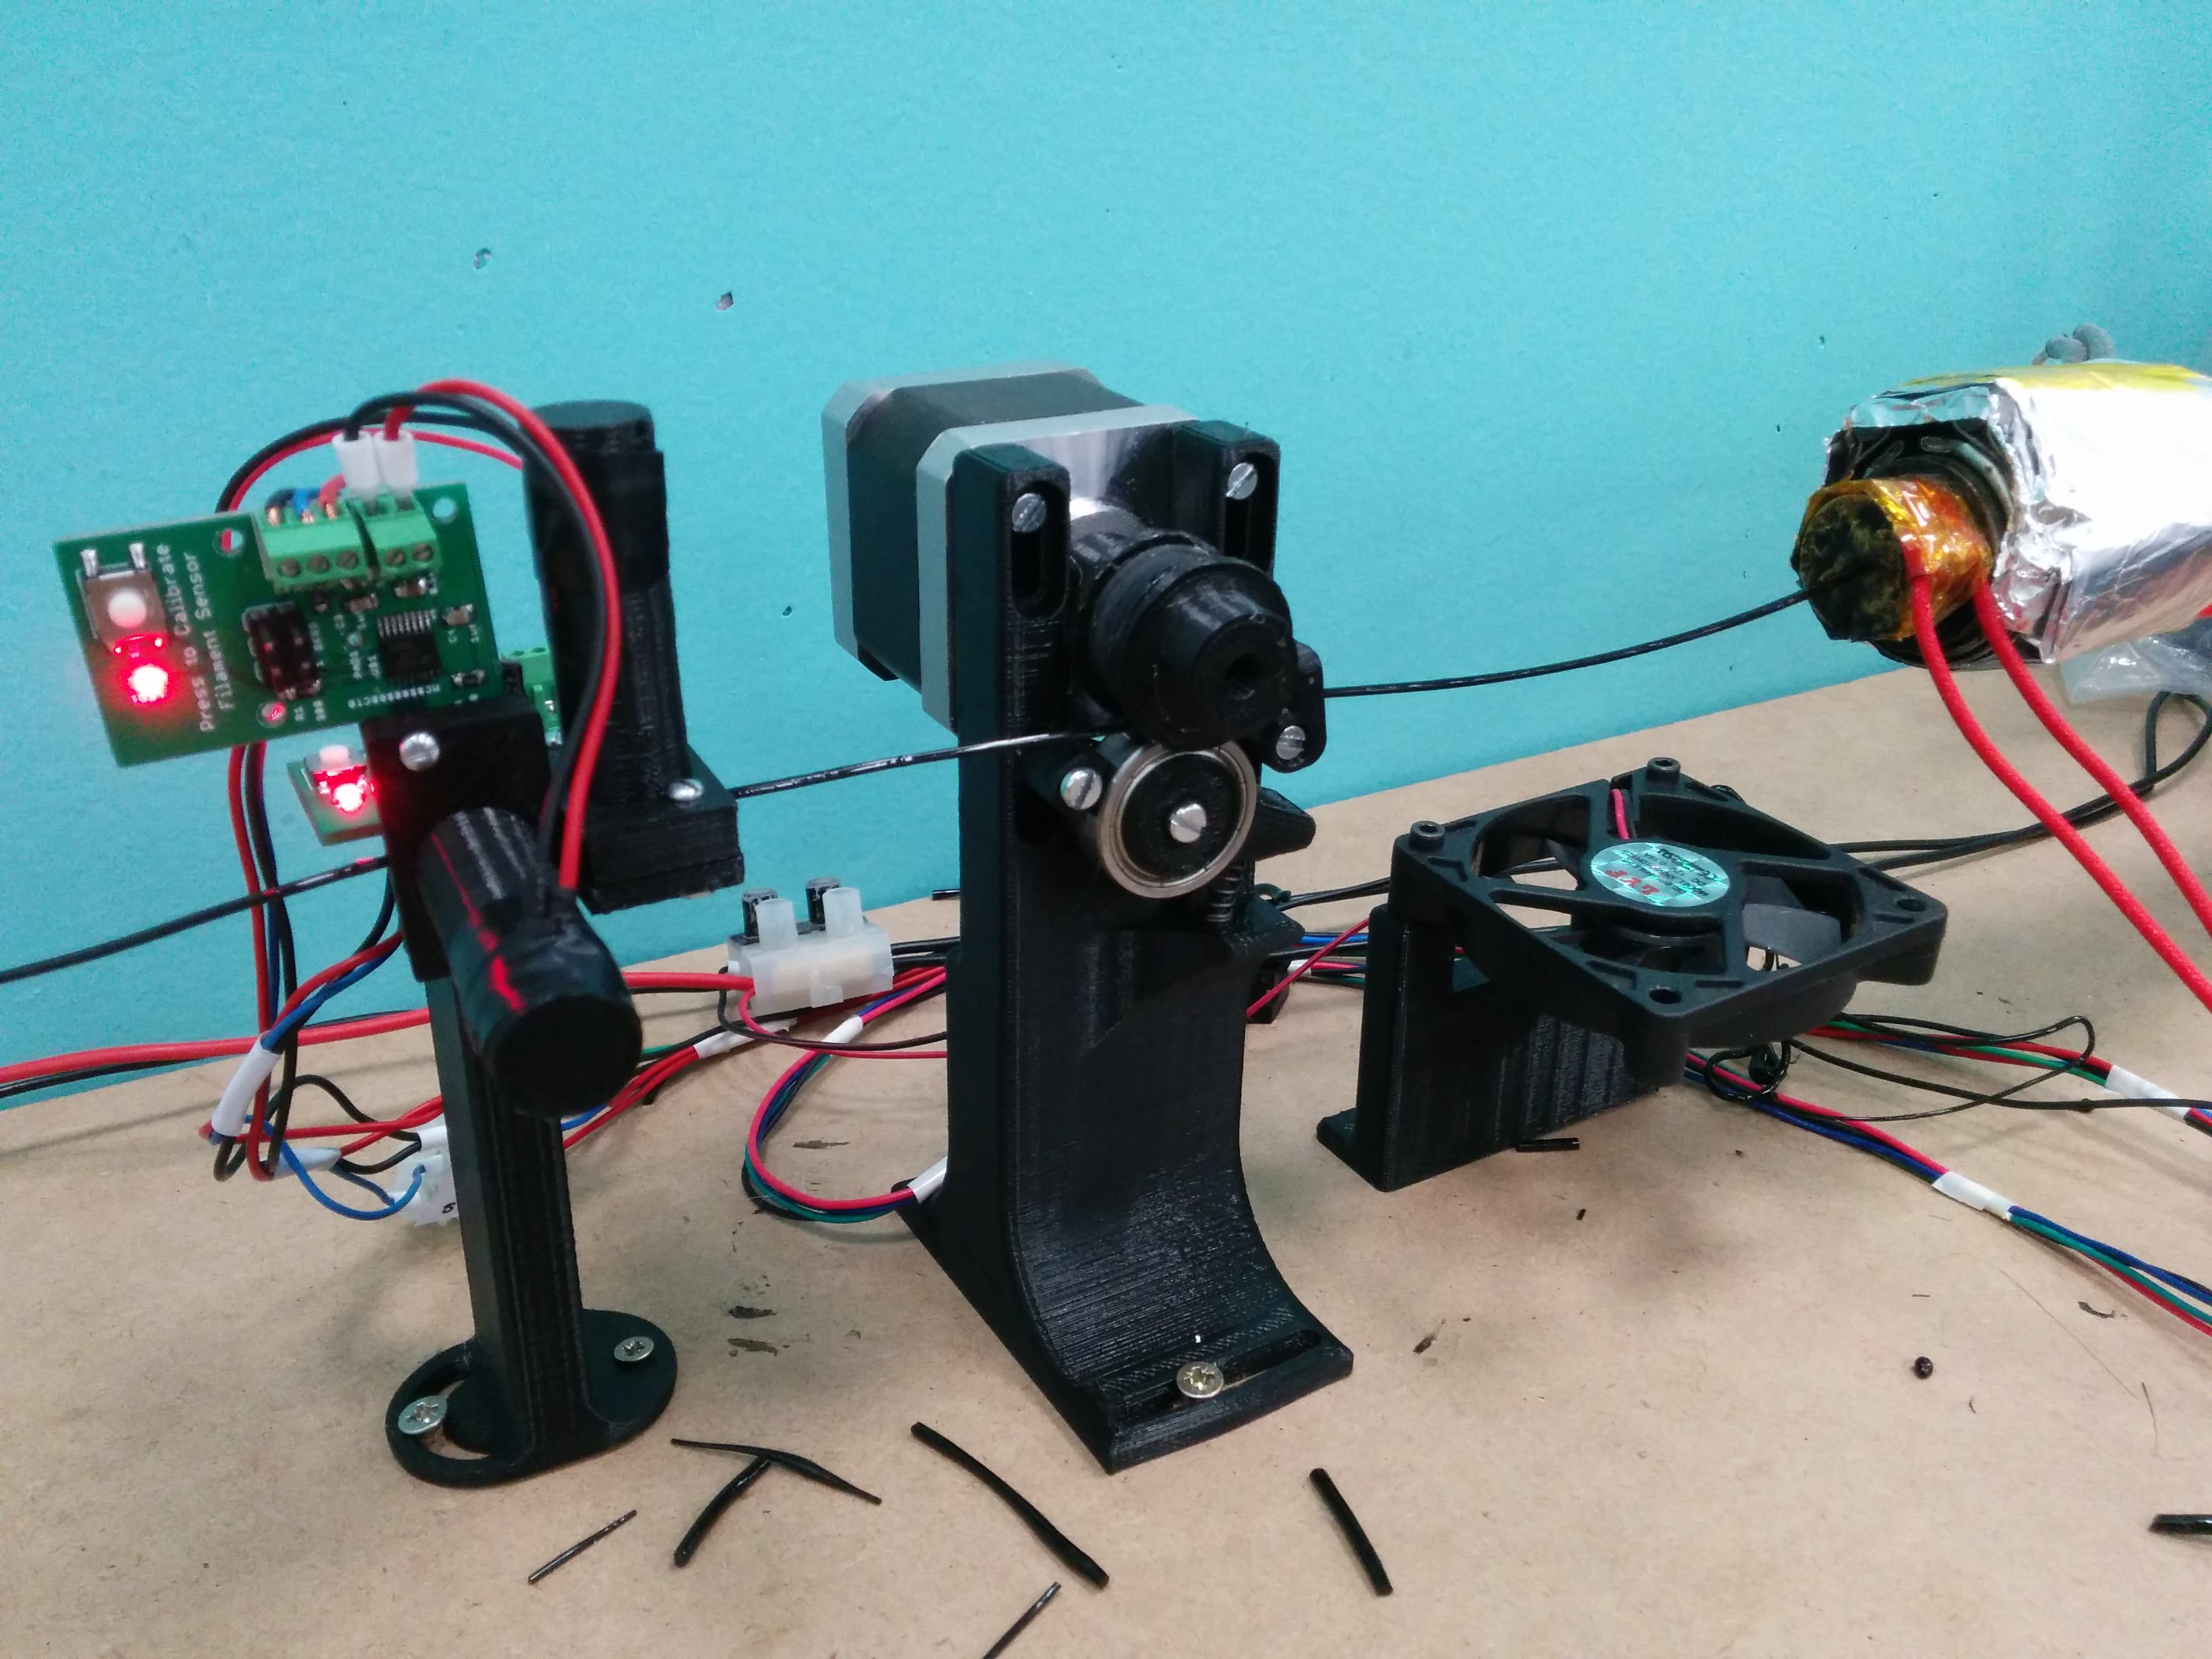
\includegraphics[width=0.6\textwidth]{images/producciones/tractora/IMG_20150709_130326.jpg}
    \caption{Montaje final filastruder-tractora-sensor}
    \label{fig:montaje_final}
\end{figure}

\subsection{Resultados}

Usando pellets reciclados, se pasa a hacer una producción de filamento, para comprobar que el diseño de la tractora es el correcto. El ensayo que se va a realizar consiste en:

\begin{itemize}
    \item{Establecer una temperatura de 135ºC en el extrusor.}
    \item{Llenar la tolva que incluye de serie la extrusora con 42gr de pellets reciclados.}
    \item{Extruir filamento registrando los datos para su posterior análisis.}
    \item{Cambiar la velocidad de tracción para comprobar la relación final en el diámetro. Se establecera una velocidad de 1RPM y 3RPM}
\end{itemize}

Se está alrededor de seis minutos extruyendo filamento, sin embargo, debido a un exceso en el diámetro del filamento, hace que este no entre por el sensor de diámetro y sea necesario parar, sin embargo podemos estudiar los datos obtenidos.
Tras el ensayo, los resultados obtenidos son los siguientes:

\begin{table}[H]
    \centering
    \begin{tabular}{cc}
               & Diámetro X \\ \hline
    Medidas    & 203        \\
    Media (mm) & 1.59       \\
    Desviación estandar & 0.25\\
    Mínimo (mm)   & 1.08       \\
    Máximo (mm)   & 2.19      
    \end{tabular}
    \caption{Datos obtenidos en el ensayo del día 20 de Julio}
    \label{tab:20007105-dat}
\end{table}


\begin{figure}[H]
    \centering
    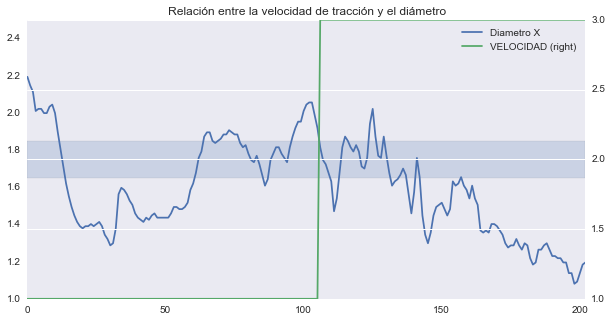
\includegraphics[width=0.99\textwidth]{images/producciones/20072015/graficas.png}
    \caption{Gráfica con los datos de la producción}
    \label{fig:2007105-graf}
\end{figure}

En la gráfica anterior vemos los datos obtenidos del diámetro del eje X. Se ve claramente, que hay una variación muy pronunciada al tener una velocidad de tracción constante, esto es un problema en el diseño de la filastruder ya que, a una velocidad de tracción constante, el diámetro debería serlo también. Durante el ensayo, se ha notado física y acústicamente que la extrusión no es constante, por ello, pensamos que el funcionamiento de la filastruder, que a simple vista parecía correcto, no puede llegar a proporcionarnos los resultados que necesitamos. Se instala un encoder mediante un imán, un sensor de efecto hall y un arduino a la filastruder, para cercionarnos de que la velocidad es constante.

\begin{figure}[H]
    \centering
    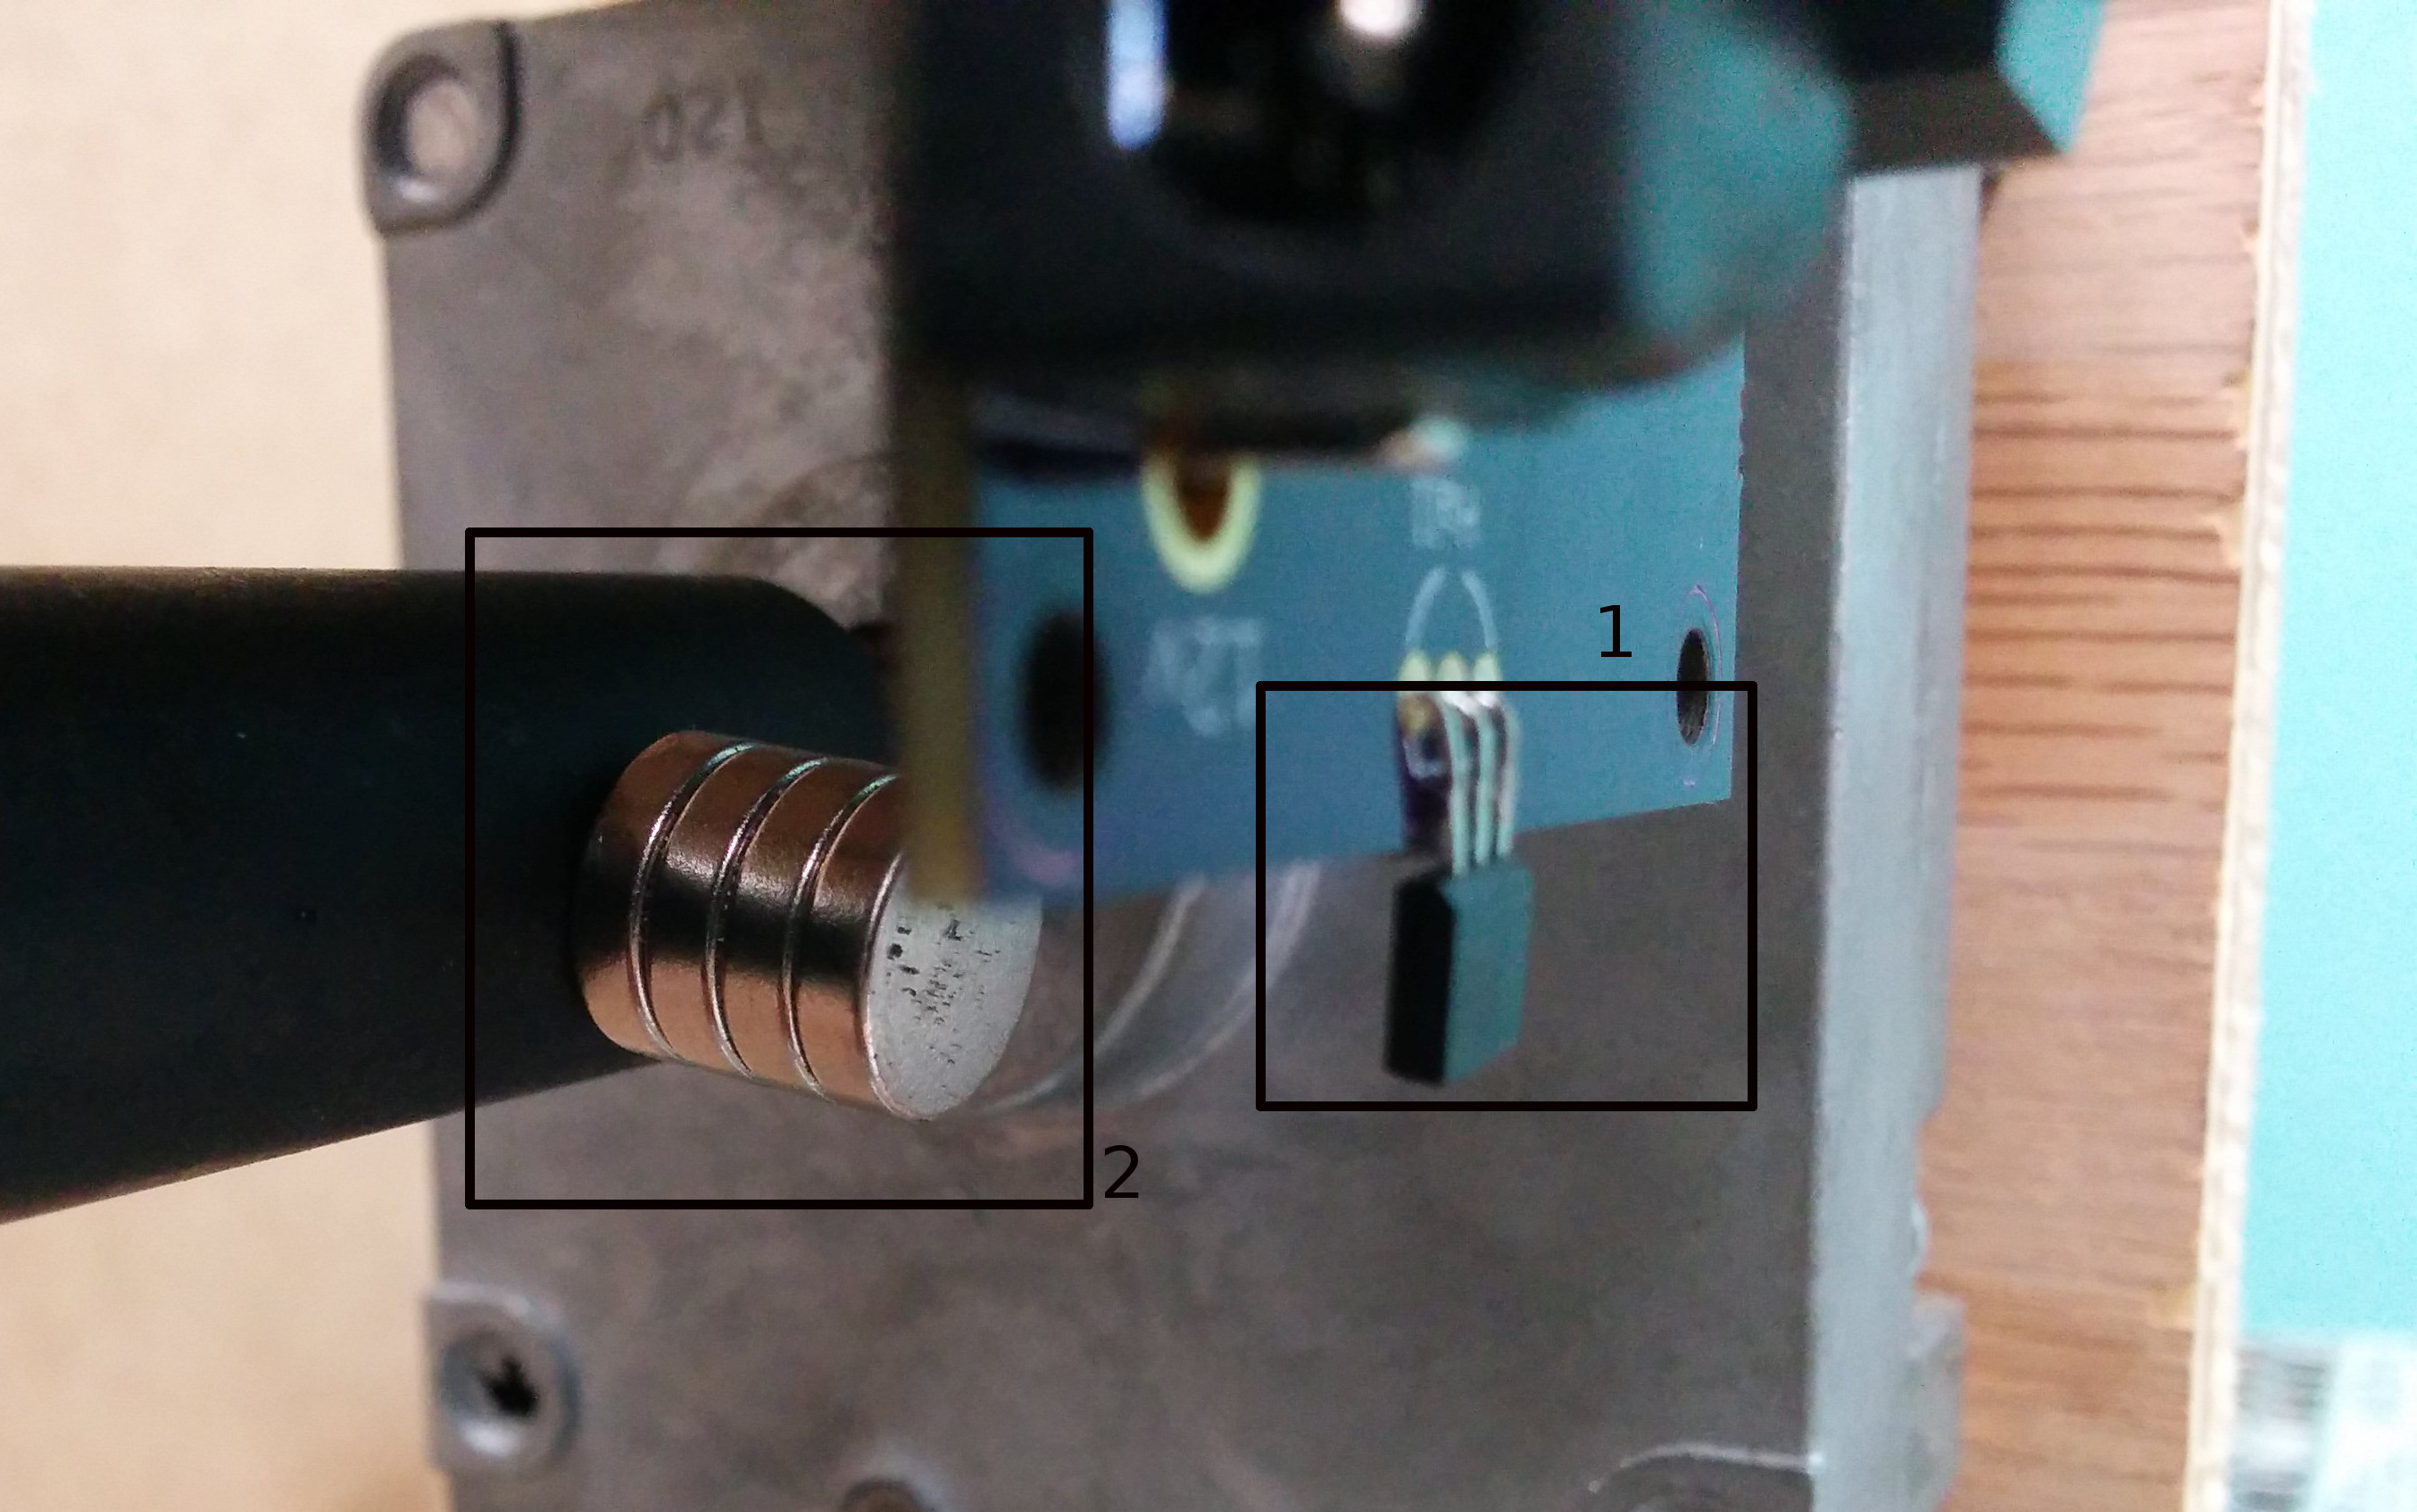
\includegraphics[width=0.8\textwidth]{images/producciones/20072015/IMG_20150721_110502.jpg}
    \caption{Encoder instalado en la filastruder.}
    \label{fig:2007105-enc}
\end{figure}

Se extruye una cantidad de filamento sin medir el diámetro, tan sólo registrando la velocidad con la que gira el husillo y los datos proporcionados son los siguientes:

\begin{figure}[H]
    \centering
    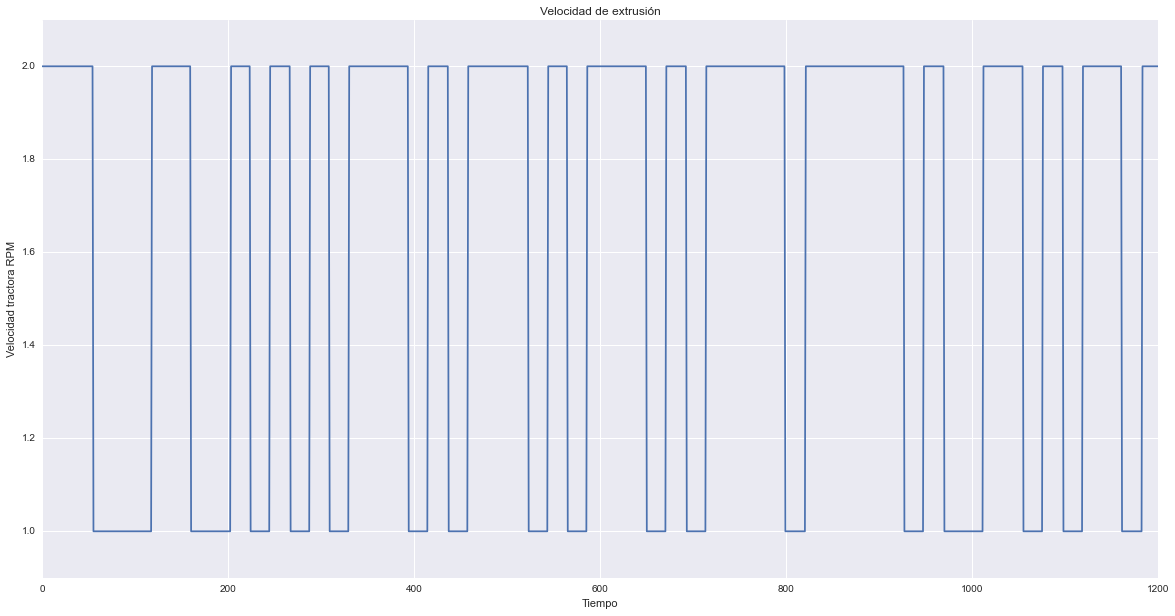
\includegraphics[width=0.99\textwidth]{images/producciones/20072015/RPM_tract.png}
    \caption{Velocidad de la extrusora.}
    \label{fig:2007105-grafenc}
\end{figure}

Vemos claramente, que la velocidad de giro no es constante, variando entre 1 y 2 RPM. El motor que hace girar el husillo está conectado directamente a 12V y no se tienen ningún control sobre él. Además mecánicamente, el motor está conectado al husillo mediante una caja reductora, la cual no podemos cambiar. Para no alargar la duración del proyecto e intentar avanzar en el control se van a tomar las siguientes medidas:

\begin{itemize}
    \item{Usar una mezcla de granza de PLA natural (70\%) con pellets reciclados de filamento (30\%) (ver imagen \ref{fig:2007105-mezc}). Se usará granza de PLA natural, el cual tiene una forma más redondeada que los pellets reciclados, haciendo más fácil el avance dentro del cañón. Se usa una mezcla con los pellets reciclados, ya que el sensor de diámetro que usamos, no funciona con filamento transparente, por ello, debemos tintar el filamento}
    \item{Antes de hacer una producción de filamento, la granza de PLA que se vaya a usar, se va a secar en un horno a una temperatura de 80ºC durante, al menos, tres horas antes de la producción. Esto es debido a que si el PLA tiene un alto porcentaje de humedad, hará que la extrusión del material no sea el adecuado, afectando directamente en el acabado final.}
    \item{Se va a diseñar una tolva de alimentación mayor, para que la capacidad de granza aumente, y se ejerza mayor presión a la entrada del extrusor, para que de ese modo, la alimentación de la granza se lo más constante posible. El tamaño de almacenamiento máximo ha pasado de 42gr a 150gr}
\end{itemize}


\begin{figure}[H]
    \centering
    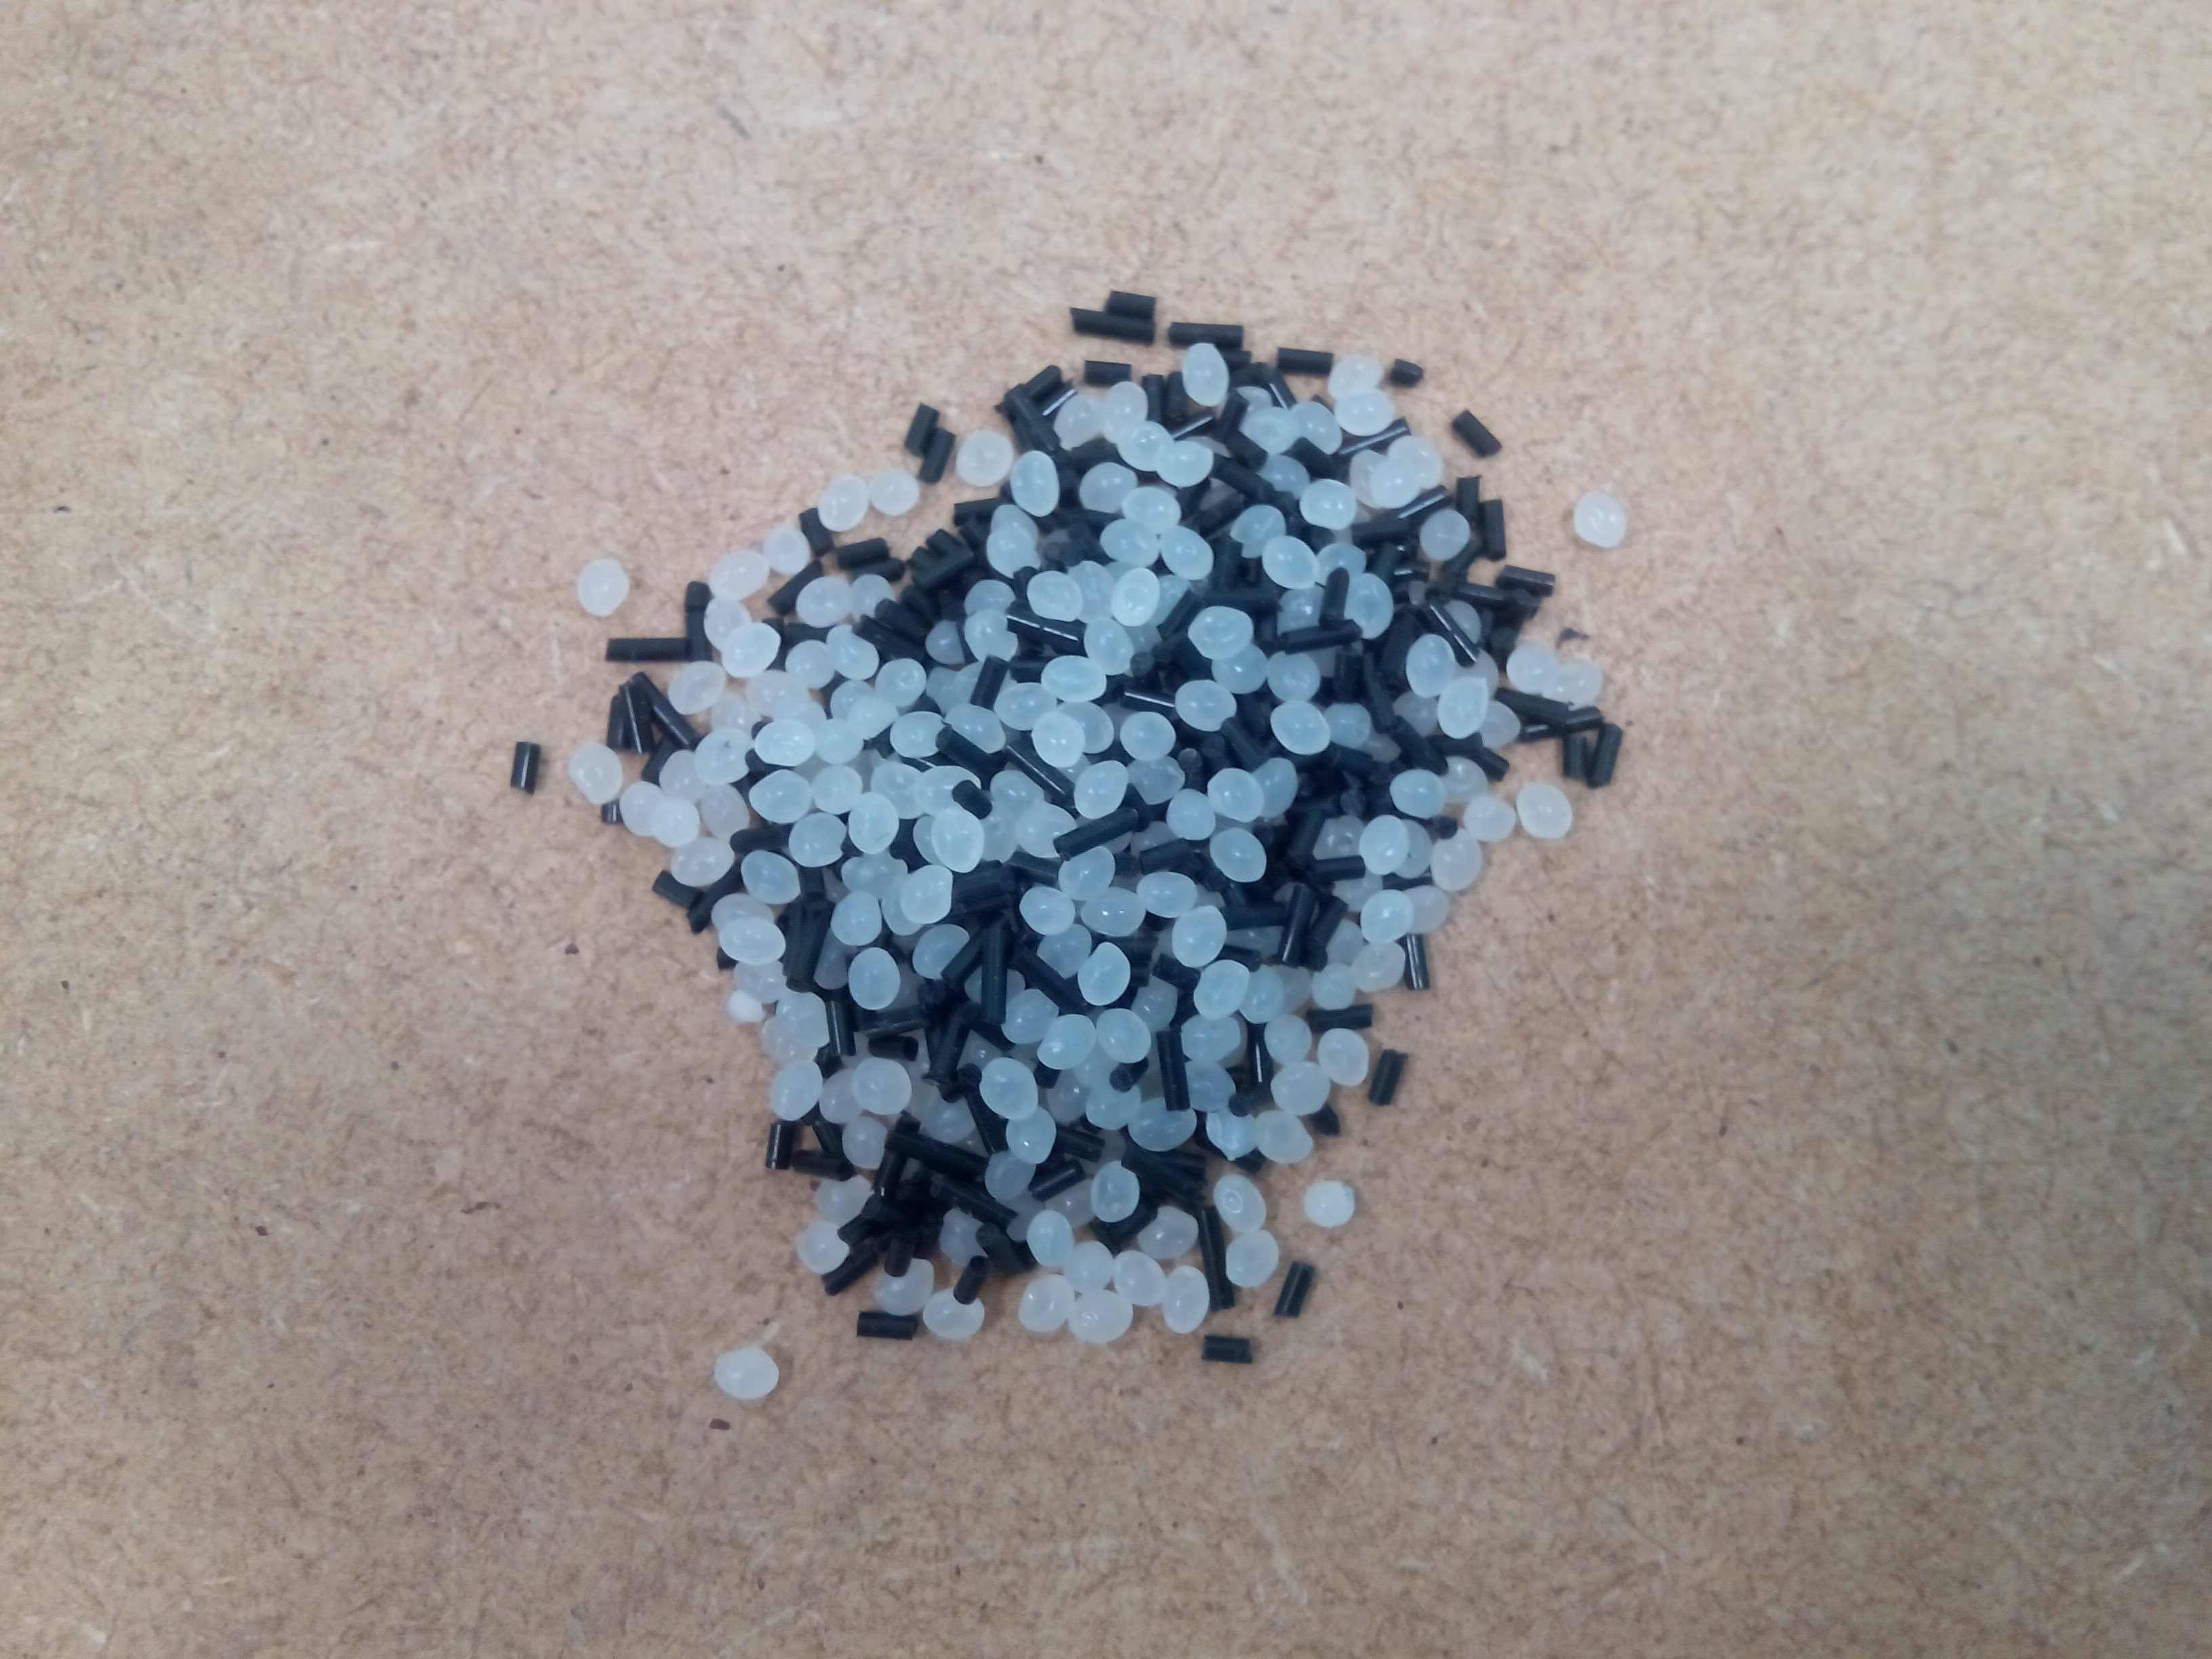
\includegraphics[width=0.6\textwidth]{images/producciones/20072015/IMG_20150903_155859.jpg}
    \caption{Mezcla de granza con pellets reciclados.}
    \label{fig:2007105-mezc}
\end{figure}

\begin{figure}[H]
    \centering
    \begin{subfigure}[b]{0.5\textwidth}
        \centering
        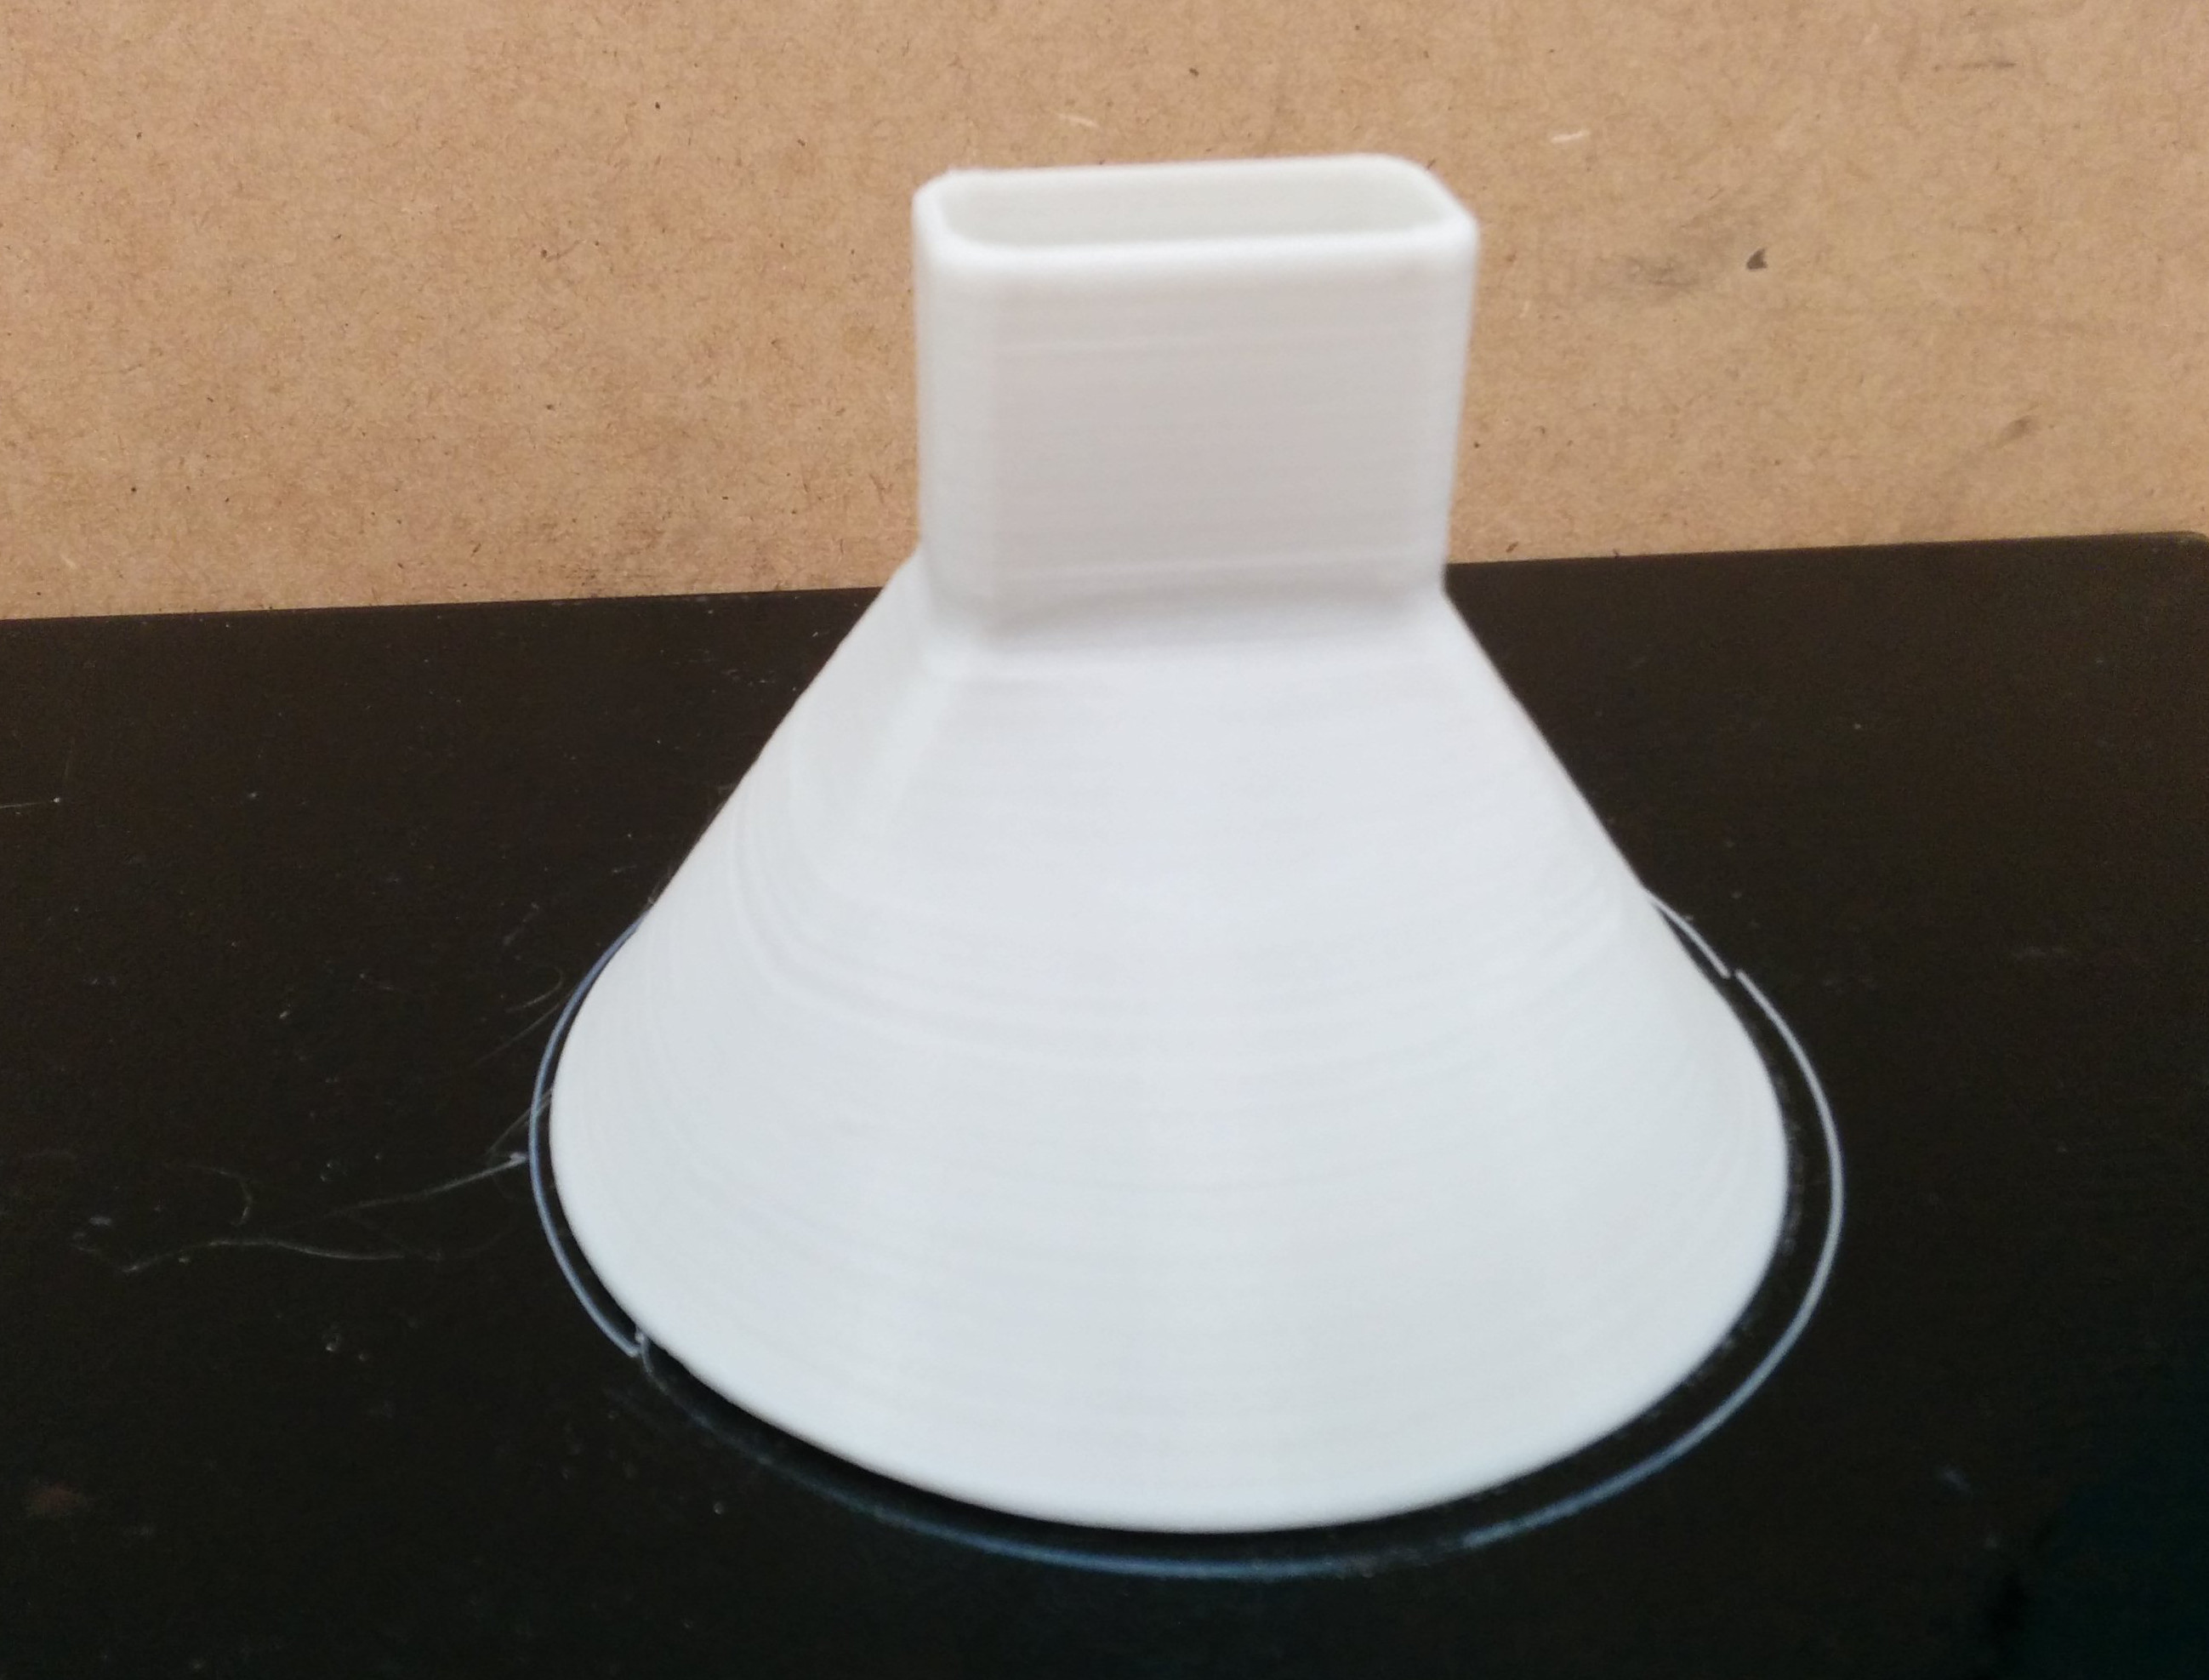
\includegraphics[width=\linewidth]{images/producciones/20072015/IMG_20150721_121831.jpg}
        \caption{Tolva impresa}
        \label{fig:tolva-impresa}
    \end{subfigure}
    ~
    \begin{subfigure}[b]{0.5\textwidth}
            \centering
        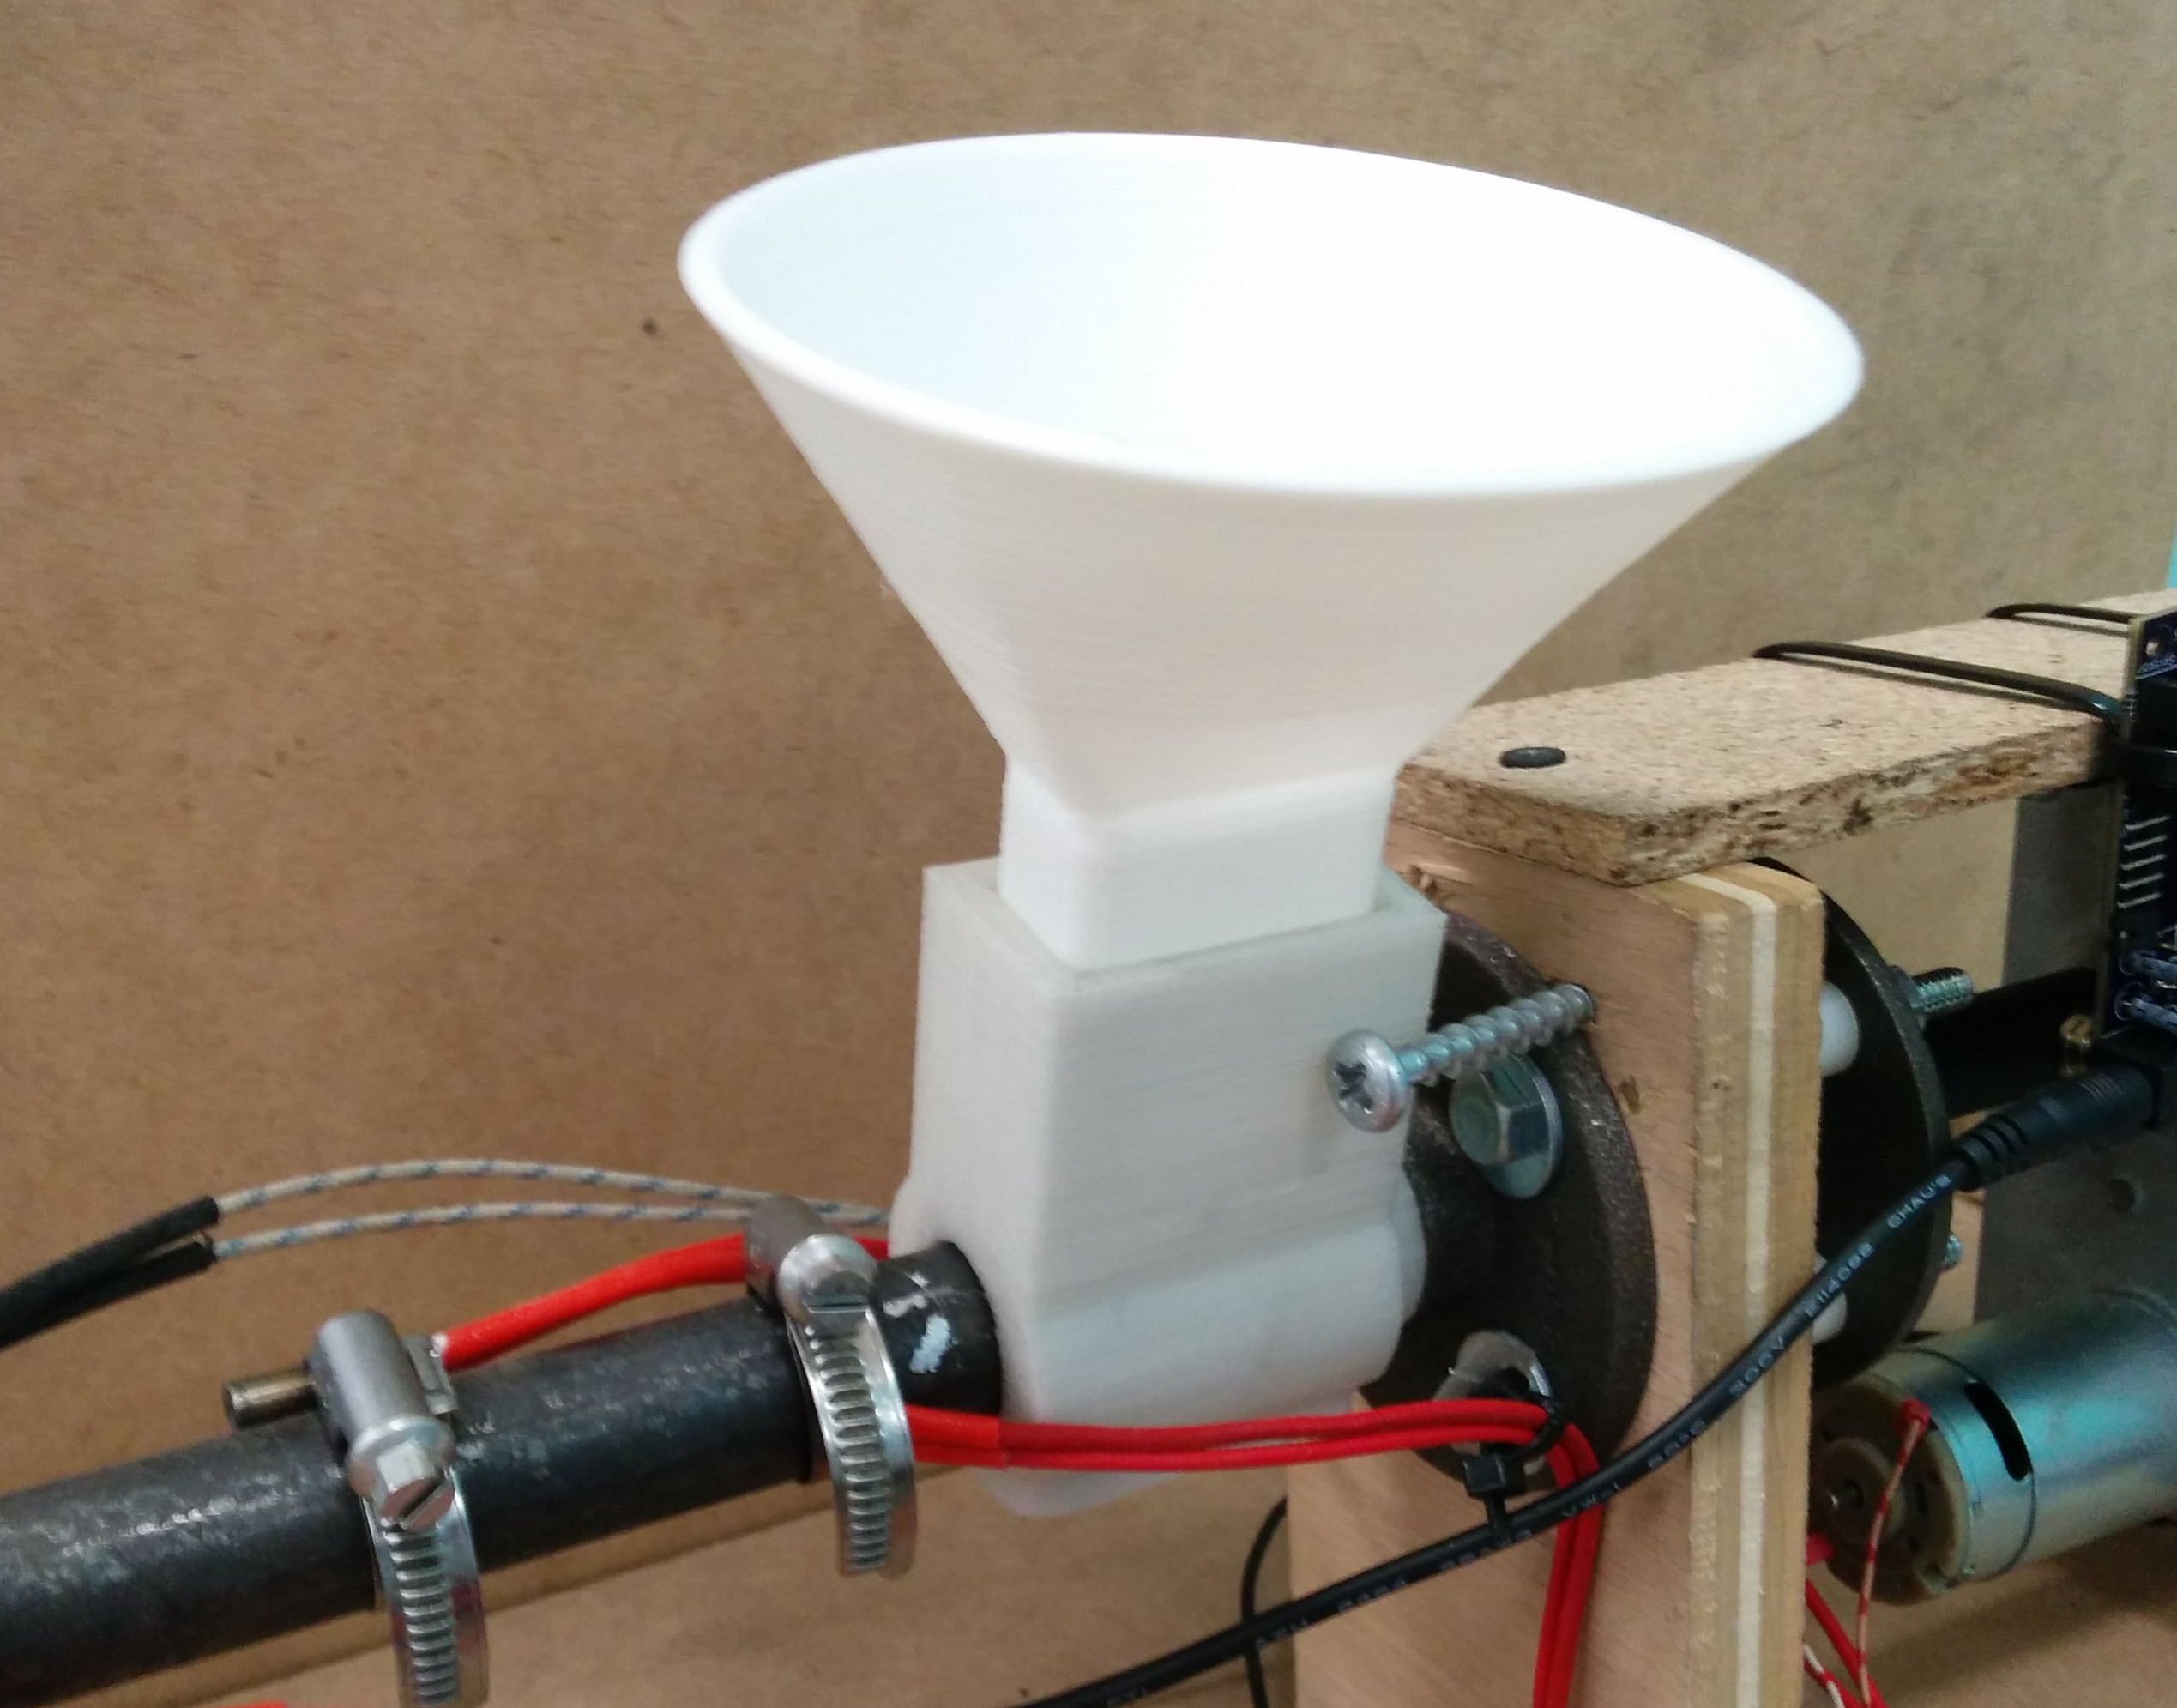
\includegraphics[width=\linewidth]{images/producciones/20072015/IMG_20150721_121904.jpg}
        \caption{Tolva montada}
        \label{fig:tolva-montada}
    \end{subfigure}
    \caption{Diseño y montaje de una tolva de mayor capacidad.}
    \label{fig:tolv_montaj}
\end{figure}

Se muestran a continuación los resultados obtenidos en el ensayo:

\begin{table}[H]
    \centering
    \begin{tabular}{ccc}
                            & Tolva Grande & Tolva pequeña \\ \hline
        Medidas               & 2000.000000  & 2000.000000   \\
        Media (mm)          & 1.63     & 1.55      \\
        Desviación estandar & 0.14     & 0.15      \\
        Mínimo (mm)             & 1.02     & 0.01      \\
        Máximo (mm)             & 2.20     & 2.40     
    \end{tabular}
    \caption{Datos del ensayo con distintas tolvas}
    \label{tab:ensa_tolvas}
\end{table}

\begin{figure}[H]
    \centering
    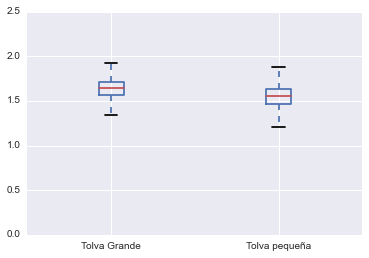
\includegraphics[width=0.8\textwidth]{images/producciones/22072015/output_6_1.png}
    \caption{Diagrama de cajas }
    \label{fig:22072015-boxplot}
\end{figure}

Como se ve en el diagrama de cajas, en el que se representa la distribución de los datos, los datos obtenidos en el ensayo con la tolva grande, son algo más estables, por lo tanto, podemos confirmar, que las medidas tomadas anteriormente para intentar mejorar la producción son acertadas, sin embargo, como se aprecia en el gráfico siguiente, se sigue teniendo una variación muy alta en el sistema, lo cual es un problema para intentar integrar un regulador del tipo PID. Por ello, se decide implementar un regulador experto para intentar controlar de forma más precisa el diámetro.

\begin{figure}[H]
    \centering
    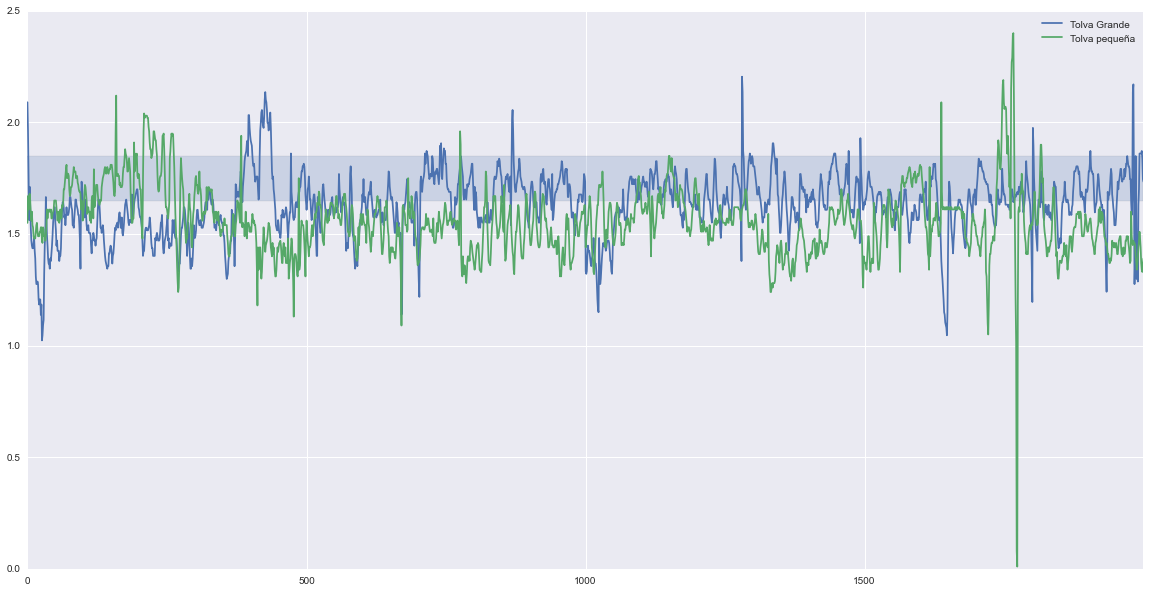
\includegraphics[width=0.99\textwidth]{images/producciones/22072015/output_7_1.png}
    \caption{Grafica con los datos obtenidos }
    \label{fig:22072015-grafica}
\end{figure}

Hasta el momento, hemos conseguido los siguientes objetivos que planteamos al principio del proyecto:

\begin{itemize}
    \item Documentación de la instrumentación de la planta.
    \item Definir la arquitectura para la comunicación del PLC y la instrumentación
    \item Definir requisitos del PLC a adquirir.
    \item Programación del PLC.
    \item Realización del armario eléctrico para montar en la fábrica.
    \item Estudio de los datos adquiridos y desarrollo del modelo teórico de la planta.
    \item Comprobar qué regulador se amolda a nuestras necesidades.
\end{itemize}

Quedándonos tan sólo:

\begin{itemize}
    \item Puesta en marcha del regulador en planta y comprobar resultados.
\end{itemize}

Además, para conseguir los dos últimos objetivos cumplidos y el objetivo que falta, se han tenido que realizar las siguientes tareas para poder conseguirlo:

\begin{itemize}
    \item Realizar una maqueta con una extrusora de fabricación casera.
    \item Conseguir reciclar PLA y que este sea funcional para extruir filamento.
\end{itemize}

En el siguiente capítulo veremos la implementación del regulador experto y analizaremos los resultados obtenidos.
